\documentclass[]{article}
\usepackage{lmodern}
\usepackage{amssymb,amsmath}
\usepackage{ifxetex,ifluatex}
\usepackage{fixltx2e} % provides \textsubscript
\ifnum 0\ifxetex 1\fi\ifluatex 1\fi=0 % if pdftex
  \usepackage[T1]{fontenc}
  \usepackage[utf8]{inputenc}
\else % if luatex or xelatex
  \ifxetex
    \usepackage{mathspec}
  \else
    \usepackage{fontspec}
  \fi
  \defaultfontfeatures{Ligatures=TeX,Scale=MatchLowercase}
\fi
% use upquote if available, for straight quotes in verbatim environments
\IfFileExists{upquote.sty}{\usepackage{upquote}}{}
% use microtype if available
\IfFileExists{microtype.sty}{%
\usepackage{microtype}
\UseMicrotypeSet[protrusion]{basicmath} % disable protrusion for tt fonts
}{}
\usepackage[margin=1in]{geometry}
\usepackage{hyperref}
\hypersetup{unicode=true,
            pdftitle={Project3},
            pdfauthor={Rongkui Han},
            pdfborder={0 0 0},
            breaklinks=true}
\urlstyle{same}  % don't use monospace font for urls
\usepackage{color}
\usepackage{fancyvrb}
\newcommand{\VerbBar}{|}
\newcommand{\VERB}{\Verb[commandchars=\\\{\}]}
\DefineVerbatimEnvironment{Highlighting}{Verbatim}{commandchars=\\\{\}}
% Add ',fontsize=\small' for more characters per line
\usepackage{framed}
\definecolor{shadecolor}{RGB}{248,248,248}
\newenvironment{Shaded}{\begin{snugshade}}{\end{snugshade}}
\newcommand{\AlertTok}[1]{\textcolor[rgb]{0.94,0.16,0.16}{#1}}
\newcommand{\AnnotationTok}[1]{\textcolor[rgb]{0.56,0.35,0.01}{\textbf{\textit{#1}}}}
\newcommand{\AttributeTok}[1]{\textcolor[rgb]{0.77,0.63,0.00}{#1}}
\newcommand{\BaseNTok}[1]{\textcolor[rgb]{0.00,0.00,0.81}{#1}}
\newcommand{\BuiltInTok}[1]{#1}
\newcommand{\CharTok}[1]{\textcolor[rgb]{0.31,0.60,0.02}{#1}}
\newcommand{\CommentTok}[1]{\textcolor[rgb]{0.56,0.35,0.01}{\textit{#1}}}
\newcommand{\CommentVarTok}[1]{\textcolor[rgb]{0.56,0.35,0.01}{\textbf{\textit{#1}}}}
\newcommand{\ConstantTok}[1]{\textcolor[rgb]{0.00,0.00,0.00}{#1}}
\newcommand{\ControlFlowTok}[1]{\textcolor[rgb]{0.13,0.29,0.53}{\textbf{#1}}}
\newcommand{\DataTypeTok}[1]{\textcolor[rgb]{0.13,0.29,0.53}{#1}}
\newcommand{\DecValTok}[1]{\textcolor[rgb]{0.00,0.00,0.81}{#1}}
\newcommand{\DocumentationTok}[1]{\textcolor[rgb]{0.56,0.35,0.01}{\textbf{\textit{#1}}}}
\newcommand{\ErrorTok}[1]{\textcolor[rgb]{0.64,0.00,0.00}{\textbf{#1}}}
\newcommand{\ExtensionTok}[1]{#1}
\newcommand{\FloatTok}[1]{\textcolor[rgb]{0.00,0.00,0.81}{#1}}
\newcommand{\FunctionTok}[1]{\textcolor[rgb]{0.00,0.00,0.00}{#1}}
\newcommand{\ImportTok}[1]{#1}
\newcommand{\InformationTok}[1]{\textcolor[rgb]{0.56,0.35,0.01}{\textbf{\textit{#1}}}}
\newcommand{\KeywordTok}[1]{\textcolor[rgb]{0.13,0.29,0.53}{\textbf{#1}}}
\newcommand{\NormalTok}[1]{#1}
\newcommand{\OperatorTok}[1]{\textcolor[rgb]{0.81,0.36,0.00}{\textbf{#1}}}
\newcommand{\OtherTok}[1]{\textcolor[rgb]{0.56,0.35,0.01}{#1}}
\newcommand{\PreprocessorTok}[1]{\textcolor[rgb]{0.56,0.35,0.01}{\textit{#1}}}
\newcommand{\RegionMarkerTok}[1]{#1}
\newcommand{\SpecialCharTok}[1]{\textcolor[rgb]{0.00,0.00,0.00}{#1}}
\newcommand{\SpecialStringTok}[1]{\textcolor[rgb]{0.31,0.60,0.02}{#1}}
\newcommand{\StringTok}[1]{\textcolor[rgb]{0.31,0.60,0.02}{#1}}
\newcommand{\VariableTok}[1]{\textcolor[rgb]{0.00,0.00,0.00}{#1}}
\newcommand{\VerbatimStringTok}[1]{\textcolor[rgb]{0.31,0.60,0.02}{#1}}
\newcommand{\WarningTok}[1]{\textcolor[rgb]{0.56,0.35,0.01}{\textbf{\textit{#1}}}}
\usepackage{longtable,booktabs}
\usepackage{graphicx,grffile}
\makeatletter
\def\maxwidth{\ifdim\Gin@nat@width>\linewidth\linewidth\else\Gin@nat@width\fi}
\def\maxheight{\ifdim\Gin@nat@height>\textheight\textheight\else\Gin@nat@height\fi}
\makeatother
% Scale images if necessary, so that they will not overflow the page
% margins by default, and it is still possible to overwrite the defaults
% using explicit options in \includegraphics[width, height, ...]{}
\setkeys{Gin}{width=\maxwidth,height=\maxheight,keepaspectratio}
\IfFileExists{parskip.sty}{%
\usepackage{parskip}
}{% else
\setlength{\parindent}{0pt}
\setlength{\parskip}{6pt plus 2pt minus 1pt}
}
\setlength{\emergencystretch}{3em}  % prevent overfull lines
\providecommand{\tightlist}{%
  \setlength{\itemsep}{0pt}\setlength{\parskip}{0pt}}
\setcounter{secnumdepth}{5}
% Redefines (sub)paragraphs to behave more like sections
\ifx\paragraph\undefined\else
\let\oldparagraph\paragraph
\renewcommand{\paragraph}[1]{\oldparagraph{#1}\mbox{}}
\fi
\ifx\subparagraph\undefined\else
\let\oldsubparagraph\subparagraph
\renewcommand{\subparagraph}[1]{\oldsubparagraph{#1}\mbox{}}
\fi

%%% Use protect on footnotes to avoid problems with footnotes in titles
\let\rmarkdownfootnote\footnote%
\def\footnote{\protect\rmarkdownfootnote}

%%% Change title format to be more compact
\usepackage{titling}

% Create subtitle command for use in maketitle
\providecommand{\subtitle}[1]{
  \posttitle{
    \begin{center}\large#1\end{center}
    }
}

\setlength{\droptitle}{-2em}

  \title{Project3}
    \pretitle{\vspace{\droptitle}\centering\huge}
  \posttitle{\par}
    \author{Rongkui Han}
    \preauthor{\centering\large\emph}
  \postauthor{\par}
      \predate{\centering\large\emph}
  \postdate{\par}
    \date{2/6/2020}

\usepackage{booktabs}
\usepackage{longtable}
\usepackage{array}
\usepackage{multirow}
\usepackage{wrapfig}
\usepackage{float}
\usepackage{colortbl}
\usepackage{pdflscape}
\usepackage{tabu}
\usepackage{threeparttable}
\usepackage{threeparttablex}
\usepackage[normalem]{ulem}
\usepackage{makecell}
\usepackage{xcolor}

\begin{document}
\maketitle

{
\setcounter{tocdepth}{2}
\tableofcontents
}
\begin{Shaded}
\begin{Highlighting}[]
\KeywordTok{library}\NormalTok{(AER)}
\end{Highlighting}
\end{Shaded}

\begin{verbatim}
## Warning: package 'AER' was built under R version 3.6.2
\end{verbatim}

\begin{verbatim}
## Loading required package: car
\end{verbatim}

\begin{verbatim}
## Loading required package: carData
\end{verbatim}

\begin{verbatim}
## Loading required package: lmtest
\end{verbatim}

\begin{verbatim}
## Loading required package: zoo
\end{verbatim}

\begin{verbatim}
## 
## Attaching package: 'zoo'
\end{verbatim}

\begin{verbatim}
## The following objects are masked from 'package:base':
## 
##     as.Date, as.Date.numeric
\end{verbatim}

\begin{verbatim}
## Loading required package: sandwich
\end{verbatim}

\begin{verbatim}
## Warning: package 'sandwich' was built under R version 3.6.2
\end{verbatim}

\begin{verbatim}
## Loading required package: survival
\end{verbatim}

\begin{Shaded}
\begin{Highlighting}[]
\KeywordTok{library}\NormalTok{(sqldf)}
\end{Highlighting}
\end{Shaded}

\begin{verbatim}
## Loading required package: gsubfn
\end{verbatim}

\begin{verbatim}
## Loading required package: proto
\end{verbatim}

\begin{verbatim}
## Loading required package: RSQLite
\end{verbatim}

\begin{Shaded}
\begin{Highlighting}[]
\KeywordTok{library}\NormalTok{(kableExtra)}
\KeywordTok{library}\NormalTok{(knitr)}
\KeywordTok{library}\NormalTok{(latexpdf)}
\end{Highlighting}
\end{Shaded}

Make suggestions to policymakers to take certain measures by discovering variables that caused the reduction or increase of traffic fatalities.

\begin{Shaded}
\begin{Highlighting}[]
\KeywordTok{data}\NormalTok{(}\StringTok{"Fatalities"}\NormalTok{)}
\NormalTok{data =}\StringTok{ }\NormalTok{Fatalities}
\KeywordTok{head}\NormalTok{(data)}
\end{Highlighting}
\end{Shaded}

\begin{verbatim}
##   state year spirits unemp   income   emppop  beertax baptist  mormon drinkage
## 1    al 1982    1.37  14.4 10544.15 50.69204 1.539379 30.3557 0.32829    19.00
## 2    al 1983    1.36  13.7 10732.80 52.14703 1.788991 30.3336 0.34341    19.00
## 3    al 1984    1.32  11.1 11108.79 54.16809 1.714286 30.3115 0.35924    19.00
## 4    al 1985    1.28   8.9 11332.63 55.27114 1.652542 30.2895 0.37579    19.67
## 5    al 1986    1.23   9.8 11661.51 56.51450 1.609907 30.2674 0.39311    21.00
## 6    al 1987    1.18   7.8 11944.00 57.50988 1.560000 30.2453 0.41123    21.00
##       dry youngdrivers    miles breath jail service fatal nfatal sfatal
## 1 25.0063     0.211572 7233.887     no   no      no   839    146     99
## 2 22.9942     0.210768 7836.348     no   no      no   930    154     98
## 3 24.0426     0.211484 8262.990     no   no      no   932    165     94
## 4 23.6339     0.211140 8726.917     no   no      no   882    146     98
## 5 23.4647     0.213400 8952.854     no   no      no  1081    172    119
## 6 23.7924     0.215527 9166.302     no   no      no  1110    181    114
##   fatal1517 nfatal1517 fatal1820 nfatal1820 fatal2124 nfatal2124  afatal
## 1        53          9        99         34       120         32 309.438
## 2        71          8       108         26       124         35 341.834
## 3        49          7       103         25       118         34 304.872
## 4        66          9       100         23       114         45 276.742
## 5        82         10       120         23       119         29 360.716
## 6        94         11       127         31       138         30 368.421
##       pop  pop1517  pop1820  pop2124 milestot unempus emppopus         gsp
## 1 3942002 208999.6 221553.4 290000.1    28516     9.7     57.8 -0.02212476
## 2 3960008 202000.1 219125.5 290000.2    31032     9.6     57.9  0.04655825
## 3 3988992 197000.0 216724.1 288000.2    32961     7.5     59.5  0.06279784
## 4 4021008 194999.7 214349.0 284000.3    35091     7.2     60.1  0.02748997
## 5 4049994 203999.9 212000.0 263000.3    36259     7.0     60.7  0.03214295
## 6 4082999 204999.8 208998.5 258999.8    37426     6.2     61.5  0.04897637
\end{verbatim}

\begin{Shaded}
\begin{Highlighting}[]
\NormalTok{?Fatalities}
\end{Highlighting}
\end{Shaded}

\begin{verbatim}
## starting httpd help server ... done
\end{verbatim}

\emph{Question:} Which factor variables change across time within each state?

\begin{Shaded}
\begin{Highlighting}[]
\NormalTok{factorchange =}\StringTok{ }\KeywordTok{sqldf}\NormalTok{(}\StringTok{"SELECT state, year, breath, jail, service FROM data"}\NormalTok{)}

\NormalTok{factorchange_table =}\StringTok{ }\KeywordTok{data.frame}\NormalTok{(}\DataTypeTok{State =} \KeywordTok{c}\NormalTok{(}\StringTok{"CO"}\NormalTok{,}\StringTok{"CT"}\NormalTok{,}\StringTok{"IL"}\NormalTok{,}\StringTok{"IN"}\NormalTok{,}\StringTok{"IA"}\NormalTok{,}\StringTok{"KS"}\NormalTok{,}\StringTok{"KY"}\NormalTok{,}\StringTok{"LA"}\NormalTok{,}\StringTok{"MS"}\NormalTok{,}\StringTok{"NV"}\NormalTok{,}\StringTok{"NH"}\NormalTok{,}\StringTok{"OH"}\NormalTok{,}\StringTok{"OR"}\NormalTok{,}\StringTok{"UT"}\NormalTok{),}
                                \DataTypeTok{Breath =} \KeywordTok{c}\NormalTok{(}\StringTok{"1982-1983"}\NormalTok{,}\StringTok{"NA"}\NormalTok{,}\StringTok{"1986 - 1987"}\NormalTok{,}\StringTok{"1983-1984"}\NormalTok{,}\StringTok{"1982-1983"}\NormalTok{,}\StringTok{"1985-1986"}\NormalTok{,}\StringTok{"1983-1984"}\NormalTok{,}\StringTok{"1982-1983"}\NormalTok{,}\StringTok{"1982-1983"}\NormalTok{,}\StringTok{"NA"}\NormalTok{,}\StringTok{"1982-1983"}\NormalTok{,}\StringTok{"NA"}\NormalTok{,}\StringTok{"NA"}\NormalTok{,}\StringTok{"NA"}\NormalTok{),}
                                \DataTypeTok{Jail =} \KeywordTok{c}\NormalTok{(}\StringTok{"NA"}\NormalTok{,}\StringTok{"1984-1985"}\NormalTok{,}\StringTok{"NA"}\NormalTok{,}\StringTok{"NA"}\NormalTok{,}\StringTok{"NA"}\NormalTok{,}\StringTok{"NA"}\NormalTok{,}\StringTok{"NA"}\NormalTok{,}\StringTok{"NA"}\NormalTok{,}\StringTok{"NA"}\NormalTok{,}\StringTok{"1982-1983"}\NormalTok{,}\StringTok{"NA"}\NormalTok{,}\StringTok{"1982-1983 & 1986 - 1987"}\NormalTok{,}\StringTok{"1983-1984"}\NormalTok{,}\StringTok{"1982-1983"}\NormalTok{),}
                                \DataTypeTok{Service =} \KeywordTok{c}\NormalTok{(}\StringTok{"NA"}\NormalTok{,}\StringTok{"1984-1985"}\NormalTok{,}\StringTok{"NA"}\NormalTok{,}\StringTok{"NA"}\NormalTok{,}\StringTok{"NA"}\NormalTok{,}\StringTok{"NA"}\NormalTok{,}\StringTok{"NA"}\NormalTok{,}\StringTok{"NA"}\NormalTok{,}\StringTok{"NA"}\NormalTok{,}\StringTok{"1982-1983"}\NormalTok{,}\StringTok{"NA"}\NormalTok{,}\StringTok{"NA"}\NormalTok{,}\StringTok{"1983-1984"}\NormalTok{,}\StringTok{"1982-1983"}\NormalTok{)}
\NormalTok{                                )}

\KeywordTok{kable}\NormalTok{(factorchange_table)}
\end{Highlighting}
\end{Shaded}

\begin{tabular}{l|l|l|l}
\hline
State & Breath & Jail & Service\\
\hline
CO & 1982-1983 & NA & NA\\
\hline
CT & NA & 1984-1985 & 1984-1985\\
\hline
IL & 1986 - 1987 & NA & NA\\
\hline
IN & 1983-1984 & NA & NA\\
\hline
IA & 1982-1983 & NA & NA\\
\hline
KS & 1985-1986 & NA & NA\\
\hline
KY & 1983-1984 & NA & NA\\
\hline
LA & 1982-1983 & NA & NA\\
\hline
MS & 1982-1983 & NA & NA\\
\hline
NV & NA & 1982-1983 & 1982-1983\\
\hline
NH & 1982-1983 & NA & NA\\
\hline
OH & NA & 1982-1983 \& 1986 - 1987 & NA\\
\hline
OR & NA & 1983-1984 & 1983-1984\\
\hline
UT & NA & 1982-1983 & 1982-1983\\
\hline
\end{tabular}

\begin{Shaded}
\begin{Highlighting}[]
\KeywordTok{library}\NormalTok{(ggplot2)}

\NormalTok{data =}\StringTok{ }\NormalTok{data[}\KeywordTok{complete.cases}\NormalTok{(data),]}
\KeywordTok{dim}\NormalTok{(data)}
\end{Highlighting}
\end{Shaded}

\begin{verbatim}
## [1] 335  34
\end{verbatim}

\begin{Shaded}
\begin{Highlighting}[]
\KeywordTok{ggplot}\NormalTok{(data, }\KeywordTok{aes}\NormalTok{(}\DataTypeTok{x =}\NormalTok{ jail, }\DataTypeTok{y =}\NormalTok{ fatal)) }\OperatorTok{+}
\StringTok{  }\KeywordTok{geom_boxplot}\NormalTok{()}
\end{Highlighting}
\end{Shaded}

\includegraphics{Project3_Connor_files/figure-latex/unnamed-chunk-4-1.pdf}

\begin{Shaded}
\begin{Highlighting}[]
\NormalTok{data[}\StringTok{'fr'}\NormalTok{] =}\StringTok{ }\NormalTok{data}\OperatorTok{$}\NormalTok{fatal}\OperatorTok{/}\NormalTok{data}\OperatorTok{$}\NormalTok{pop}\OperatorTok{*}\DecValTok{10000}

\KeywordTok{ggplot}\NormalTok{(data, }\KeywordTok{aes}\NormalTok{(}\DataTypeTok{x =}\NormalTok{ jail, }\DataTypeTok{y =}\NormalTok{ fr)) }\OperatorTok{+}
\StringTok{  }\KeywordTok{geom_boxplot}\NormalTok{()}
\end{Highlighting}
\end{Shaded}

\includegraphics{Project3_Connor_files/figure-latex/unnamed-chunk-5-1.pdf}

\begin{Shaded}
\begin{Highlighting}[]
\KeywordTok{ggplot}\NormalTok{(data, }\KeywordTok{aes}\NormalTok{(}\DataTypeTok{x =}\NormalTok{ drinkage, }\DataTypeTok{y =}\NormalTok{ fr)) }\OperatorTok{+}
\StringTok{  }\KeywordTok{geom_point}\NormalTok{()}
\end{Highlighting}
\end{Shaded}

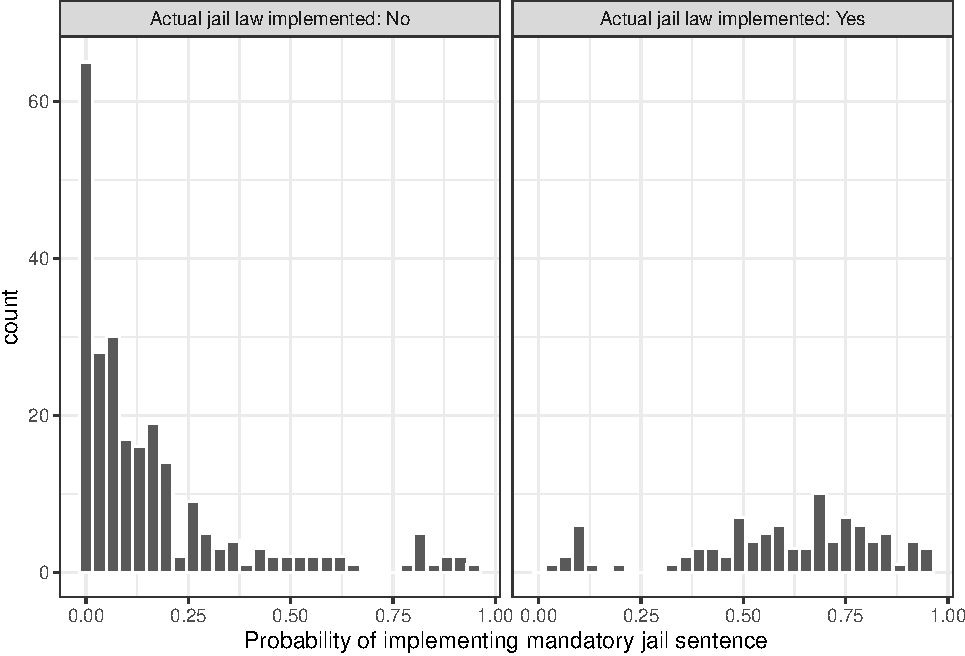
\includegraphics{Project3_Connor_files/figure-latex/unnamed-chunk-6-1.pdf}

\begin{enumerate}
\def\labelenumi{\arabic{enumi}.}
\item
  Explore this dataset and generate summary statistics (in forms of tables or plots) that you find crucial for your own interest, or for convincing the policymakers.
\item
  Consider only the full dataset from 1982 to 1988, propose a regression model to study whether having a mandatory jail sentence is associated with reduced traffic fatalities. In particular, you need to
\end{enumerate}

\begin{itemize}
\tightlist
\item
  specify your model,
\item
  state the assumptions required,
\item
  fit the model with appropriate methods,
\item
  conduct model diagnostics and/or sensitivity analysis,
\item
  and discuss causal interpretation of the proposed models.
\end{itemize}

\begin{enumerate}
\def\labelenumi{\arabic{enumi}.}
\setcounter{enumi}{2}
\item
  Conclude your analysis results. You may want to test a hypothesis, construct a confidence interval, or draw a confidence band.
\item
  Explain the implications of your results to policymakers who know little about statistics. Make suggestions if you want to.
\end{enumerate}


\end{document}
